\chapter[General Aptitude]{General Aptitude}

This document contains short notes of the most expected topics from the aptitude section in the GATE Examination. Weightage of General Aptitude in GATE Exam is 15 marks.
It also contains some concepts, formulas and tricks to solve the problems.

\section{Quantitative Aptitude}

\textbf{Face Value} - The Face Value of a digit in a numeral is its own value, at whatever place it may be Ex: 6843 face value of 6 is 6\\
\textbf{Place Value} - The Place Value of a digit 'd' in position n of a numeral is \(d * 10^{n-1}\).\\ In numeral 1856, the place value of 8 is 8*100 = 800\\
\textbf{Perfect Number} - Sum of Factors of a number (except the number itself) equals to the given number. Ex: \(6=1+2+3\)\\
\textbf{Irrational Number} - Numbers expressed in decimal would be in non-terminating and non-repeating form, are called irrational numbers. Ex: \(\sqrt{2}, \sqrt{3}, \sqrt{5}, \sqrt{7}, \pi, e \) \\
\textbf{Co-Prime or Relative Prime} - HCF between two numbers is 1.\\
Ex: (2, 3), (8, 9)\\
\textbf{Twin Prime} - Two prime numbers whose difference is 2. \\Ex: (3, 5), (5, 7)\\
\\\textbf{Note: 1} is Unique Number, neither prime nor composite.


\subsection{Unit Digit}
The last digit of a numeral is called Unit Digit.\\
Ex: Unit digit of 56516 is 6.\\
If a number K is raised to power 'n' and the unit digit of K is U, then Unit digit of \(K^n\) will only depend on \(U^n\)


\subsection{Cyclicity of a Unit Digit}
\textbf{Case 1} - If U = 0, 1, 5, 6, then \(U^n\) = 0, 1, 5, 6.\\
\textbf{Case 2} - If U = 4, 9 then cyclicity is 2
\[4^{even} = 6,  4^{odd} = 4, 9^{even} = 1, 9^{odd} = 9\]
\textbf{Case 3} - If U = 2, 3, 7, 8, then cyclicity is 4
\[U^p = U^{p/4 + k} = U^k = U_v\]
Example: Unit digit of \(7^{786}\) \[7^{786} = 7^{784/4 + 2} = 7^2 = 9\]


\subsection{Divisibility Rule}
\textbf{Divisible by 2}, if the unit digit is 0, 2, 4, 6, 8.\\
\textbf{Divisible by 3/9}, if the sum of digits divisible by 3/9.\\
\textbf{Divisible by 4}, if the last two digits divisible by 4.\\
\textbf{Divisible by 5}, if the unit digit is 0 or 5.\\
\textbf{Divisible by 6}, if it is divisible by 2 and 3.\\
\textbf{Divisible by 7/13}, divide the number into group of 3 digits find the difference between odd and even place, if the result is 0 or divisible by 7/13 then it is divisible.\\
\textbf{Divisible by 8}, if the last three digits divisible by 8.\\
\textbf{Divisible by 10}, if the unit digit is 0.\\
\textbf{Divisible by 11}, if the difference between sum of digits in odd place \& sum of digits in even place is 0 or 11 then it is divisible.


\subsection{Test for a Number to be Prime}
Let P be the given Number and let n be the smallest counting number such that \(n^2 \geq P\)\\
Now, test whether p is divisible by any of the prime numbers less than or equal to n. If the given number is divisible it is not prime else prime.


\subsection{Eucliden or Division Algorithm}
If we divide a given number with another number, then
\[Dividend = Divisor * Quotient + Remainder\]


\subsection{Factors Terminology}
Let N be a real positive number, to find the total number of factors the number should be expressed in terms of prime number as given below.
\[N = 2^a * p_1^b * p_2^c * p_3^d \ldots\]
Total Number of factors (TNF) = \((a+1)(b+1)(c+1)(d+1)...\)\\
Total Number of odd factors (TNOF) = \((b+1)(c+1)(d+1)...\)\\
Total Number of even factors (TNEF) = TNF - TNOF\\
Total Number of prime factors (TNPF) = \(a+b+c+d+...\)\\
Total Number of distinct prime factors = no of primes

\subsection{HCF and LCM}
For two numbers \(LCM*HCF=N1*N2\)\\
If a Numbers or ratio of numbers are given for the LCM (N), then use
\(LCM(2k, 3k, 4k, 5k) = N\) \textbf{Note} K can be taken out.

\subsection{Highest power of 'p' in n!}
\[= \lfloor \frac{n}{p} \rfloor + \lfloor \frac{n}{p^2} \rfloor + \lfloor \frac{n}{p^3} \rfloor + \ldots \ till \ 0\]
In simple terms Adding products of Division table. If the number is not prime then reduce it to prime and find products for each primes.


\subsection{Number of Zeros in n!}
Number of Zeros can be represented by highest power of 10. The highest power will be always less for large number \(2^m 5^n; n<m\). Use 5 Divison table.


\subsection{Remainder Theorem}
\begin{fleqn}
    \[1.\ R\left( \frac{n1*n2*n3\ldots}{d}\right) = R\left(\frac{r1*r2*r3\ldots}{d}\right)\]
    \[2.\ R\left( \frac{a^n}{d}\right)=R\left(\frac{a*a*a\ldots}{d}\right) = R\left(\frac{r^n}{d}\right)\]
    \[3.\ R\left( \frac{(a+1)^n}{a}\right)=1\]
    \[4.\
    R\left( \frac{a^n}{a+1} \right) = 
    \begin{cases}
        a,& \text{if n is odd}\\
        1,& \text{if n is even}
    \end{cases}
    \]
Example: Find the Remainder of 16*24*33 when divided by 5.
\[R\left(\frac{16*24*33}{5}\right) = R\left(\frac{1*4*3}{5}\right) = R(3)\]
\end{fleqn}


\subsection{Arithemetic Progression (A.P)}
If a difference between two terms of a series is d then it is defined as given below.
\begin{fleqn}
\[a,\ a+d,\ a+2d,\ \ldots\]
\[n^{th} \text{term of series } T_n = a + (n-1)d\]
\[\text{Sum of n terms } S_n = \frac{n}{2}\left[ a+ T_n \right] = \frac{n}{2} \left[ 2a + (n-1)d \right]\]
\end{fleqn}


\subsection{Geometric Progression (G.P)}
If a difference between two terms of a series is r then it is defined as given below.
\begin{fleqn}
\[a,\ ar,\ ar^2,\ ar^3,\ \ldots \]
\[n^{th} \text{term of series } T_n = ar^{n-1}\]
\[\text{Sum of n terms } S_n = a\left( \frac{1 - r^n}{1-r} \right) or\ a \left( \frac{r^n-1}{r-1} \right)\]
\[
\text{Sum of } \infty \ terms =
\begin{cases}
    \frac{a}{1-r}, &|r| < 1\\
    \infty, &|r| \geq 1 
\end{cases}
\]
\end{fleqn}


\subsection{Ratio}
The ratio of two quantities a and b in same units, is the fraction \(\frac{a}{b}\) and we write it as \(a:b\). Multiplication or Divison of each term of a ratio by the same non-zero number does not affect the ratio.\\ 
\textbf{Note:} a is antecedent and b is consequent


\subsection{Proportions}
The equality of two ratios is called proportion.
If \(a:b=c:d,\text{ then } a:b::c:d\) \\
Here a and d are extermes, while b and c are mean terms
\[\text{Product of means} = \text{Product of Extermes} \]
\[b*c=a*d\]


\subsection{Percentage Results}
\begin{enumerate}
    \item If a certain value of p increases by x\% , then increased value of p = (100 + x)\% of p. \\
    \item If a certain value of p decreases by x\% , then decreased value of p = (100 - x)\% of p. \\
    \item If the price of a commodity increases by R\% then the reduction in consumption so as not to increase the expenditure is 
    \[\left[ \frac{R}{100+R}*100\right]\% \]
    \item If the price of a commodity decreases by R\% then the increase in consumption so as not to decrease the expenditure is 
    \[\left[ \frac{R}{100-R}*100\right]\% \]
    \item Let the population of a town be P now and suppose it increases at the rate of R\% per annum, then:
    \begin{fleqn}
        \[\text{1. Population after n years}=P\left( 1+\frac{R}{100}\right)^n \]
        \[\text{2. Population n years ago}=\frac{P}{\left( 1+\frac{R}{100}\right)^n} \]
    \item Let the present value of a machine be P. Suppose it depreciates at the rate of R\% per annum, then:
        \[\text{1. Value of the machine after n years}=P\left( 1-\frac{R}{100}\right)^n \]
        \[\text{2. Value of the machine n years ago}=\frac{P}{\left( 1-\frac{R}{100}\right)^n} \]
    \end{fleqn}
\end{enumerate}


\subsection{Mixtures and Allegations}
\textbf{Alligation} - It is the rule that enables us to find the ratio in which two or more ingredients at the given price must be mixed to produce a mixture of a desired price.\\
\textbf{Mean Price} - The Cost Price(C.P) of a unit quantity of the mixture.\\
\textbf{Rule of Alligation} - If two ingredients are mixed, then
\[\left(\frac{\text{Quantity of cheaper}}{\text{Quantity of dearer}} = \frac{\text{(C.P of dearer) - (Mean price)}}{\text{(Mean price) - (C.P of cheaper)}}\right)\]
\[\text{(Cheaper Quantity):(Dearer Quantity)}=(d-m):(m-c)\]
\textbf{Result} - Suppose a container contains x units of liquid from which y units are taken out and replaced by water.\\
After n operations, the quantity of pure liquid \( = \left[x\left(1-\frac{y}{x} \right)^n \right]\) units.
\begin{figure}[h!]
    \centering
    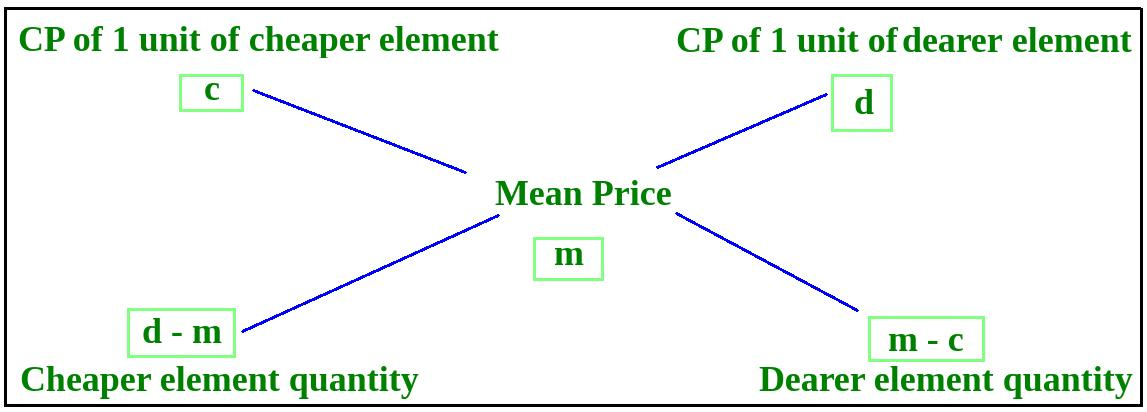
\includegraphics[width=\linewidth]{images/alligation.png}
\end{figure}


\subsection{Profit and Loss}
If a product is sold, then the dealer obtains either gain or loss.
\begin{table}[h!]
    \centering
    \setlength{\tabcolsep}{3em}
    \tabulinesep=3mm
    \begin{tabu}{l l}
    Gain = SP - CP                    & Loss = CP - SP                    \\
    \(Gain\% = \frac{SP-CP}{CP}*100\) & \(Loss\%=\frac{CP-SP}{CP}*100\)   \\
    \(S.P=\frac{100+Gain\%}{100}*CP\) & \(S.P=\frac{100-Loss\%}{100}*CP\) \\
    \(C.P=\frac{100}{100+Gain\%}*SP\) & \(C.P=\frac{100}{100-Loss\%}*SP\)
    \end{tabu}
\end{table}

Selling a product with false value.
\[\%profit= \frac{True - False}{False}*100\]


\subsection{Partnership}
When two or more than two persons run a business jointly, they are called partners and the deal is know as partnership.\vspace{0.2cm}\\
\textbf{Simple Partnership} A simple parthership is the one in which the capitals of all the partners are invested for the same time. In this partnership, the gain or loss is distributed among the partners in the ratio of their investments.\\
Suppose A and B invest Rs.x and Rs.y respectively for a year in a business, then at the end of the year.\\
\[\text{(A's share of profit):(B's share of profit) = x : y}\]
\textbf{Compound Partnership} A compound partnership is the one in which the capitals of the partners are invested for different time periods.\\
In this partnership the equivalent capitals are calculated for a unit of time by taking (capital x number of units of time). Now, gain or loss is divided in the ratio of these capitals.\\
Suppose A invests Rs.x for p months and B invest Rs.y for q months, then
\[\text{(A's share of profit):(B's share of profit) = xp : yq}\]


\subsection{Simple and Compound Interest}
\begin{fleqn}
\[Simple\ Interest=\frac{Pnr}{100}, \text{p - Amount, n - time period, r - rate of interest}\]
\[Annual\ Compound\ Interest=P\left(1+\frac{r}{100} \right)^n\]
\[Half-Yearly\ Compound\ Interest=P\left(1+\frac{r/2}{100} \right)^{2n}\]
\[Quartely\ Compound\ Interest=P\left(1+\frac{r/4}{100} \right)^{4n}\]
\end{fleqn}
{\textbf{\large{Results}}}\\
\begin{enumerate}
    \item when interest is compounded annually but time is in fraction, \(a\frac{b}{c}\)
    \[Compound\ Interest=P\left(1+\frac{r}{100} \right)^a*\left(1+\frac{r\frac{b}{c}}{100} \right)\]
    \item when rates are different for different years, say \(R_1\%, R_2\%, R_3\%\) for 1st, 2nd and 3rd year respectively.
    \[Compound\ Interest=P\left(1+\frac{R_1}{100} \right)*\left(1+\frac{R_2}{100} \right)*\left(1+\frac{R_3}{100} \right)\]
    \item Present worth of Rs. x due in n years is given by:
    \[Present\ Worth=\frac{x}{\left(1 + \frac{R}{100}\right)^n}\]
\end{enumerate}


\subsection{Time \& Work}
\textbf{Efficiency} - Work done in unit time \(e=\frac{w}{t}\)
If A takes \(N_1\) days and B takes \(N_2\) days to complete the same work, then their efficiency is \(\frac{w}{N_1}\) and \(\frac{w}{N_2}\).\\
\[Efficiency\ of\ (A+B)=\frac{w}{N_1}+\frac{w}{N_2}=w\frac{N_1+N_2}{N_1N_2}\]
\[Time\ taken\ by\ (A+B)=\frac{N_1N_2}{N_1+N_2}\]
\[Work=Men*Days*time*efficiency\]
\textbf{Pipes and Cisterns} - In pipes and cistern, if a pipe empty a tank then it is known as negative work.


\subsection{Speed, Time \& Distance}
\[speed=\frac{distance}{time}; \ \ \ \ 1\ km/hr=\frac{5}{18}m/s; \ \ 1\ m/s=\frac{18}{5}m/s\]
\[Average Speed = \frac{Total Distance}{Total Time}=\frac{2s_1s_2}{s_1+s_2}\]
Relative speed of A and B if they are travelling in same direction is \\\( R_s=S_a - S_b\)\\
Relative speed of A and B if they are travelling in opposite direction is \( R_s=S_a + S_b\)\\
If a person is travelling is velocity s kmph for the time period of t. If he increases the speed by x to reduce the time taken as y, then the equation is given by
\[ys + xt = |x*y|\]
\textbf{\large{Problems on Trains}}\\
If two trains(or bodies) start at same time from point A and B towards each other and after crossing they take a and b hrs in reaching B and A respectively, then \(A's\ Speed:B's\ Speed=\sqrt{b}: \sqrt{a}\)\\
\begin{figure}[h]
    \centering
    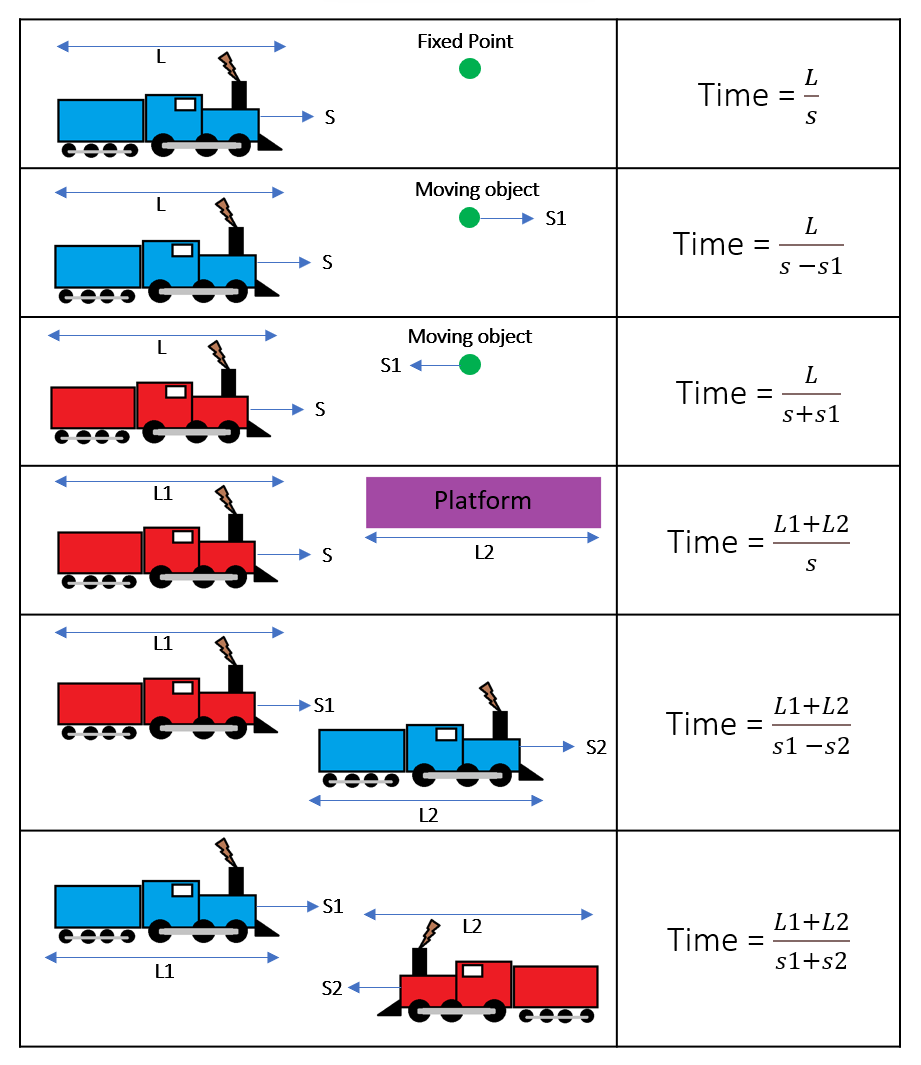
\includegraphics[scale=0.60]{images/train-problems.png}
\end{figure}

\textbf{\large{Problems on Boats}}
\[Upstream: S_u = S_b - S_w,\ Downstream:S_u = S_b + S_w,\ Stillwater: S_u = S_b \]

\subsection{Permutations \& Combinations}
\textbf{Permutation} - The different arrangements of a given number of things by taking some or all at a time are called permutations.\\
\textbf{Combination} - Each of the different groups or selections which can be formed by taking some or all at a time, is called combination.\vspace{0.2cm}\\
\textbf{Results}
\begin{enumerate}
    \item Arrangement of 'k' items out of 'n' without repetition is given by\\
    $\Perm{n}{k}=\frac{n!}{(n-k)!}$
    \item Arrangement of 'n' items out of 'n' is given by
    $\Perm{n}{n}=n!$
    \item Arrangement of a word with length n and two repetitive letters of length a and b is\\
    $\frac{\Perm{n}{n}}{\Perm{a}{a}*\Perm{b}{b}}=\frac{n!}{a!*b!}$
    \item selection of 'k' things out of 'n' is given by
    $\Comb{n}{k}=\frac{n!}{k!(n-k)!}$;  $\Comb{10}{3}=\frac{10*9*8}{1*2*3}$
    \item Division of 'n' items among 'r' persons
        \begin{enumerate}
            \item If a person can receive zero (or more thing) $\Comb{n+r-1}{r-1}$ \((0\leq r\leq n)\)
            \item If a person can receive atleast one item $\Comb{n-1}{r-1}$ \((1\leq r\leq n)\)
        \end{enumerate}
\end{enumerate}


\subsection{Probability}
\textbf{Random Experiment} - An experiment in which all the possible outcomes (Sample Space) are known and the exact output cannot be predicted in advance, is called a random experiment.\\
\textbf{Probability of Occurrence of an Event}\\
Let S be the sample space and let E be an Event. Then,
\[P(E)=\frac{n(E)}{n(S)}\]
\textbf{Results}
\textbf{Binomial Probability Law}\\
For a single event 'r' to happen in 'n' independent trials is given by
\begin{center}
$\Comb{n}{r}$\((P(E))^r(P(\overline{E}))^{n-r}\)
\end{center}
\textbf{Results}
\begin{enumerate}
    \item P(S) = 1
    \item \(0 \leq P(E) \leq 1\)
    \item For any events A and B, \(P(A \cup B) = P(A) + P(B) - P(A \cap B)\)
    \item \(P(\overline{A})=1-P(A)\)
\end{enumerate}

\subsection{Mensuration \& Geometry}
\textbf{Results}
\begin{enumerate}
    \item In cyclic quadrilateral, the sum of opposite angle is 180 degree.
    \item the radial line to the tangent at point of contact is perpendicular to the tangent.
    \item the perpendicular from the center of the circle to a chord bisects the chord.
    \item Common pythagoras triplets are (3, 4, 5), (5, 12, 13), (8, 15, 17)
\end{enumerate}
\begin{figure}[h!]
    \centering
    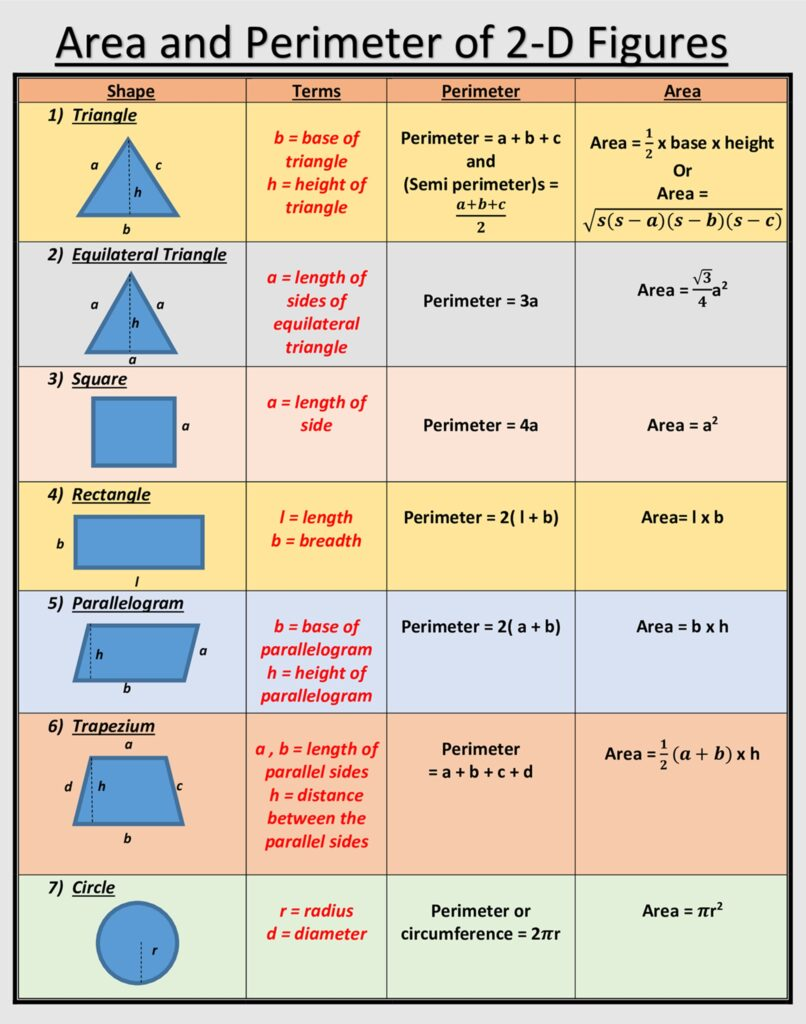
\includegraphics[scale=0.70]{images/area-perimeter.png}
\end{figure}
\begin{figure}[h!]
    \centering
    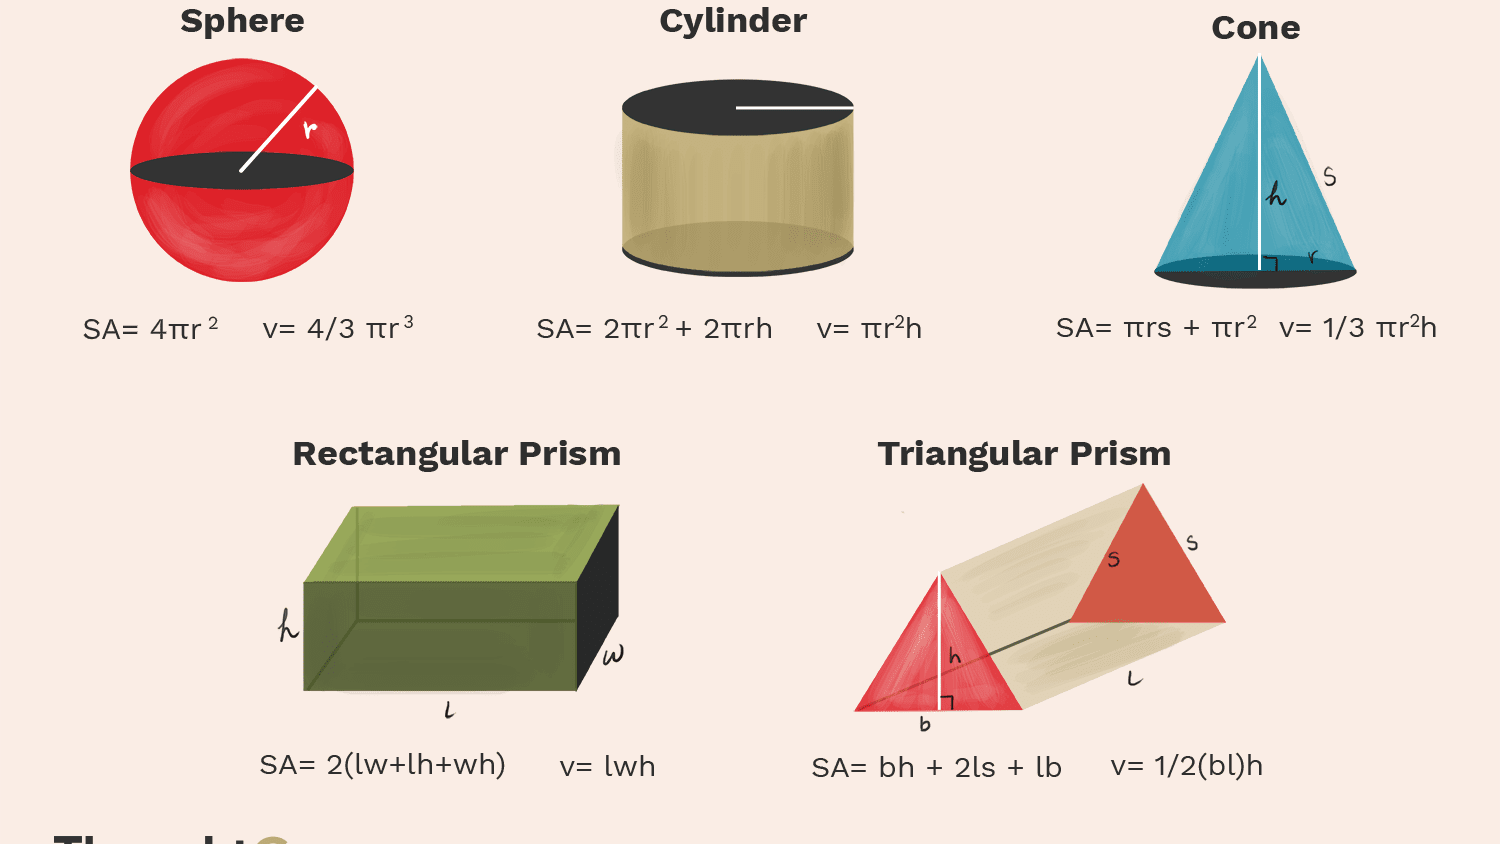
\includegraphics[width=\linewidth]{images/volume-and-surface-area.png}
\end{figure}


\subsection{Important Formulas}
\textbf{Lograthmic}\\
\begin{fleqn}
\[log(mn)=log(m)+log(n) \ \ \ \ \ \ log\left(\frac{m}{n}\right)=log(m)-log(n) \ \ \ \ \ n\log(m)=log(m)^n \]
\[log_m(m)=1 \ \ \ \ \ \ \ \ \ \ \ \ \ \ \ \ \ log(1)=0\ \ \ \ \ \ \ \ \ \ \ \ \ \ \ \ \ \ \ \ \ \ log_ba=\frac{log_{10}a}{log_{10}b}\]
\[log(x) \ \forall \ x > 1; \ \text{No of digits = characteristic + 1}\]
\[characteristic = \lfloor log(x)\rfloor \ \text{mantissa = decimal} \]
\textbf{Example}
\[log(0.36)=-0.44,\text{ characteristic}=\lfloor-0.44\rfloor = -1, \ mantissa=1-0.44=0.56\]
\[log(0.36)=\bar{1}.56\]
\[log(2.4)=0.38,\text{ characteristic}=\lfloor0.38\rfloor = 0, \ mantissa=0.38\ \text{No of digits} = 1\]
\textbf{Exponential } \(e^0 = 1;\ e^{-\infty}=0;\ e^\infty=\infty\)\vspace{0.2cm}\\
\end{fleqn}
\textbf{Algebric}\\
\(1. (a+b)^3 = a^3 + b^3 + 3ab(a+b) \ \ \ \ \)
\(2. a^3+b^3=(a+b)(a^2+b^2-ab)\) \\
\(3. (a-b)^3 = a^3 - b^3 - 3ab(a-b) \ \ \ \ \)
\(4. a^3-b^3=(a-b)(a^2+b^2+ab)\) \\
\(5. (a+b+c)^2=a^2+b^2+c^2+2(ab+bc+ca)\) \\
\(6. a^3+b^3+c^3-3abc=(a+b+c)(a^2+b^2+c^2-ab-bc-ca)\) \\


\section{Analytical Aptitude}
\subsection{Syllogism}
If two or more statements and conclusions are given in the problem. Considering the given statements are true, we need to find whether the conclusion logically follows the statement.\vspace{0.2cm}\\
\textbf{Venn Diagram Method}\\
1. Statement: If All B's are A's. Conclusion: Some A's are B's.\\
2. Statement: Some B's are A's. Conclusion: Some A's are B's.\\
3. Statement: All A's are B's. Some C's are A's. Conclusion is true if it satisfy all the conditions.
\begin{figure}[h!]
    \centering
    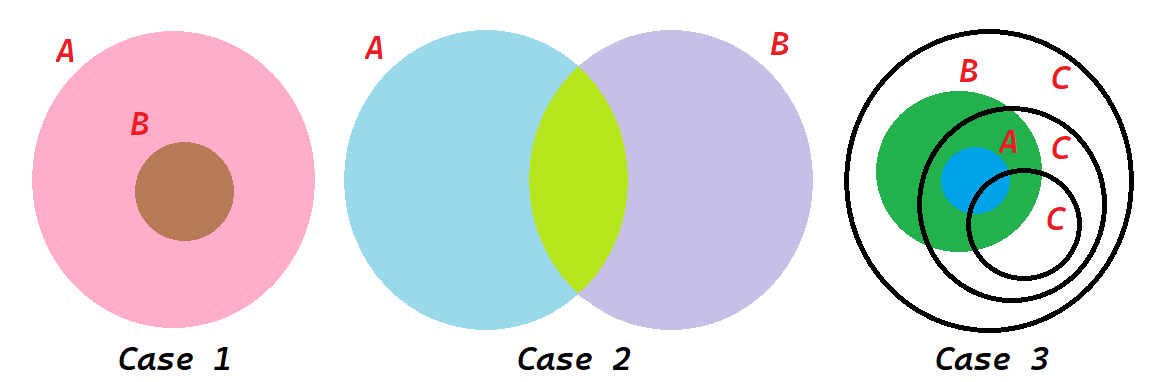
\includegraphics[width=\linewidth]{images/syllogism.png}
\end{figure}


\subsection{Blood Relations}
If the speaker points out a person and then explains the relation between the speaker and the person, then try to minimize the given statement to solve the problem else use family tree method. Refer the attached Images.\vspace{0.2cm}\\
\textbf{Family Tree Method}
\begin{figure}[h!]
    \centering
    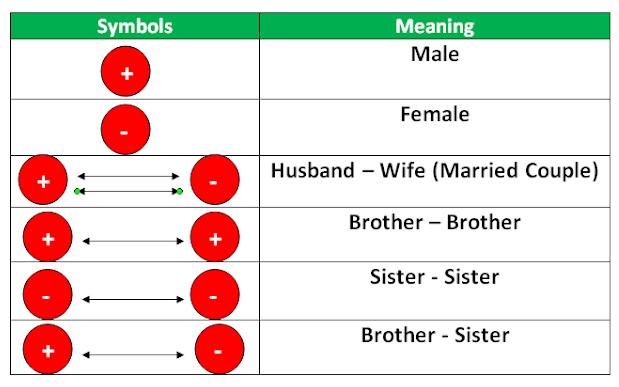
\includegraphics[scale=0.525]{images/blood-relation-family-tree-2.png}
\end{figure}
\begin{figure}[h!]
    \centering
    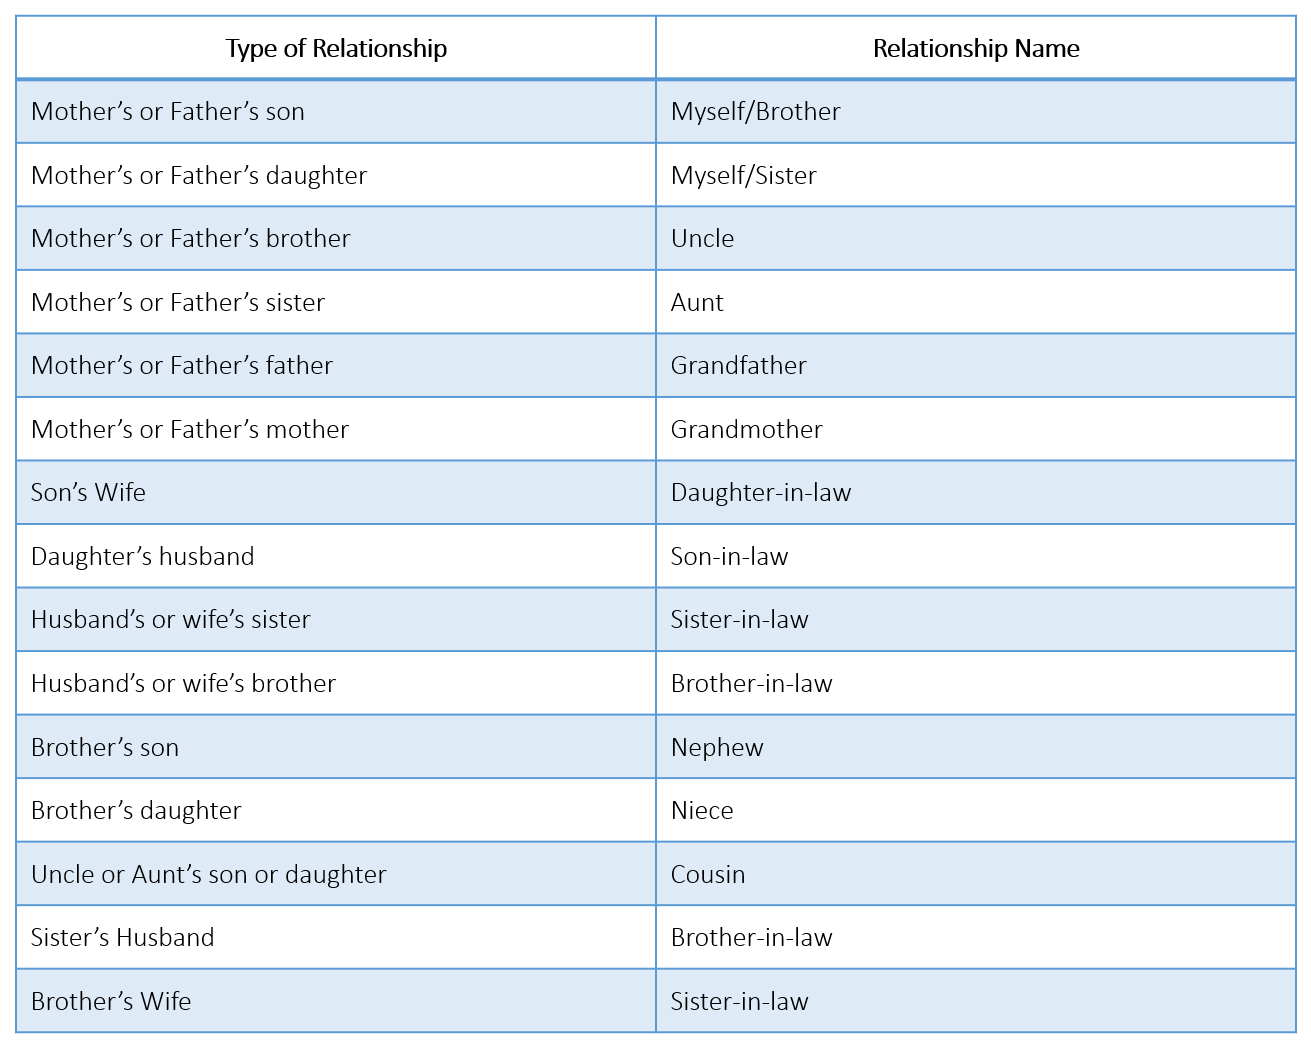
\includegraphics[width=\linewidth]{images/blood-relation.png}
\end{figure}


\subsection{Clocks and Calendars}
\begin{fleqn}
\textbf{Clock Time} if the image of the clock is mirrored or water.
\[Mirror\ time=11:60-hh:mm\]
\[
Water\ time=
\begin{cases}
    |18:30-hh:mm|, &\text{if minutes} \leq 30\\
    |18:90-hh:mm|, &\text{if minutes} > 30
\end{cases}
\]
\end{fleqn}
\textbf{Angle} between the hour hand and minute hand is given by the formula.
\[\theta = |30H-\frac{11}{2}M|\]
If a clock is showing time behind the actual time at t1 and the clock is showing time ahead of the actual time at t2. Clock showed the correct time between t2 and t1. To find that sum up the total hours and find the rate at which the time changes.\\
\textbf{Leap year} - If the current year is century year, then it should be divisible by 400 else divisible by 4.\vspace{0.2cm}\\
\textbf{Find the day} - If a day is given and we need to find the n'th day we use odd days method.\vspace{0.2cm}\vspace{0.2cm}\\
\textbf{Odd days} is number of days other than complete week.\vspace{0.2cm}\\
\[Odd\ days=R\left[\frac{\text{Total No of days}}{7} \right]\]
If Odd days is 0, then the day is the given day else add the odd days after the given day.\vspace{0.2cm}\\
\textbf{Calendar Matching}
\begin{enumerate}
    \item Add Odd days of the year from the given year till 7.
    \item if the year next to that is leap and the actual year is not leap or viceversa, Repeat Step 1, else the next year is matching year.
\end{enumerate} 


\subsection{Directions}
Draw follow-up diagram to the question to solve it. Apply pythagoras theorem if neccessary.
\begin{figure}[h!]
    \centering
    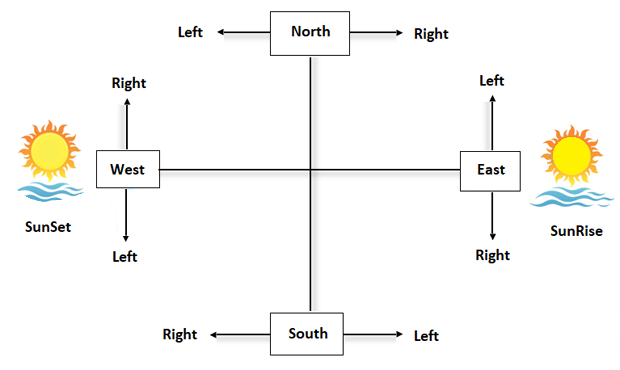
\includegraphics[width=\linewidth]{images/direction-sense.png}
\end{figure}


\section{Spatial Aptitude}
Mirror \& Water Image, Paper Cutting \& Folding, Pattern Finding, Figure Completion, Rotation objects and Seating Arrangement are not included as it does not have concepts, formulas and tricks as they only needs practice to solve it.
\subsection{Figure Counting}
\begin{enumerate}
    \item Number of squares in a square of "n" rows x "n" columns.
    \[1^2+2^2+3^2+\ldots\ldots+n^2=\frac{n(n+1)(2n+1)}{6}\]
    \item Number of rectangles in a square of "n" rows x "n" columns.
    \[1^3+2^3+3^3+\ldots\ldots+n^3=\left[ \frac{n(n+1)}{2}\right]^2\]
    \item Number of squares in a rectangle of "m" rows x "n" columns\
    \[=mn+(m-1)(n-1)+(m-2)(n-2)+\ldots.till\ 0\]
    \item Number of rectangles in a rectangle of "m" rows x "n" columns
    \[=(1+2+3+\ldots.+m)(1+2+3+\ldots.+n)\]
\end{enumerate}


\subsection{Coding-Decoding}
If a certain word is coded using a logic, then it can be used to code (or) decode another word.\\
To remember a position of a letter quickly, Remember the word \textbf{EJOTY}.\\
Position of E,J,O,T,Y = \textbf{5,10,15,20,25}


\section{Verbal Aptitude}
Verbal Aptitude is all about standard written english, at first make sure you have understood parts of speech and the rules of it. This section is the vast area and requires constant practice to get marks. Choose the Appropriate word, Complete the sentence and Error Spotting requires us to understand the common rules of english grammer like preposition, verb and article usage.


\subsection{Important Points to Note}
\begin{itemize}
    \item Conditionals
        \begin{enumerate}
            \item If + Present,...........future
            \item If + Past,................would + verb
            \item If + Past perfect,....would + have + past participle
            \item If + were,................would + verb // Irrespective of previous rules
        \end{enumerate}
    \item superflucity - excessive usage of pronoun/noun
    \item Reading Comprehension - Do not answer from out of context
    \item Courses of Action - No Assumption/opinions should be considered
\end{itemize}